\documentclass[12pt]{article}
\usepackage[utf8]{inputenc}
\usepackage{float}
\usepackage{amsmath}
\usepackage{graphicx}

\usepackage[hmargin=3cm,vmargin=6.0cm]{geometry}
\topmargin=-2cm
\addtolength{\textheight}{6.5cm}
\addtolength{\textwidth}{2.0cm}
\setlength{\oddsidemargin}{0.0cm}
\setlength{\evensidemargin}{0.0cm}
\usepackage{indentfirst}
\usepackage{amsfonts}

\graphicspath{ {./images/} }


\begin{document}

\vspace*{\fill}
\begingroup
\centering

\section*{Student Information}

Name : Yaşar Cahit Yıldırım \\

ID : 2310647 \\

\endgroup
\vspace*{\fill}

\newpage

\section*{Answer 1}
Population varience $\sigma$'s are unknown. We will use Student's $t$ distribution since the sample sizes are normally distributed and small. Assuming variances between old and young populations are equal. $s_p$ is the pooled standard deviation and:
$$s_p = \sqrt{\frac{(n-1)s_X^2 + (m-1)S_Y^2}{n+m-2}} = \
    \sqrt{\frac{(19-1)(0.96)^2 + (15-1)(1.12)^2}{19+15-2}} = \
    \sqrt{\frac{34.1504}{32}} = 1.0672$$

Degree of freedom is $n+m-2 = 19+15-2 = 32$.

\subsection*{Part a)}
Target confidence interval is $95\%$, so $\alpha$ is $0.05$ and $t_{\alpha/2} = 2.037$. So the margin (let's call it $m$) is:
$$m = t_{\alpha/2} \cdot s_p\sqrt{\frac{1}{n} + \frac{1}{m}} = 2.037\cdot 1.0672 \sqrt{\frac{1}{19} + \frac{1}{15}} = 0.7509$$

So the confidence interval is:
$$\bigg[\overline{X} - \overline{Y} - m, \overline{X} - \overline{Y} + m \bigg] = \bigg[3.375 - 2.05 - 0.7509, 3.375 - 2.05 + 0.7509 \bigg] = \bigg[0.5741
, 2.0759 \bigg]$$


\subsection*{Part b)}
Target confidence interval is $90\%$, so $\alpha$ is $0.1$ and $t_{\alpha/2} = 1.694$. So the margin (let's call it $m$) is:
$$m = t_{\alpha/2} \cdot s_p\sqrt{\frac{1}{n} + \frac{1}{m}} = 1.694\cdot 1.0672 \sqrt{\frac{1}{19} + \frac{1}{15}} = 0.6244$$

So the confidence interval is:
$$\bigg[\overline{X} - \overline{Y} - m, \overline{X} - \overline{Y} + m \bigg] = \bigg[3.375 - 2.05 - 0.6244, 3.375 - 2.05 + 0.6244 \bigg] = \bigg[0.7006
, 1.9494 \bigg]$$

\subsection*{Part c)}
We need to establish an interval of $(3, 5]$ in order to answer this. Consider hypothesis' $H_0 : \mu = 3$ and $H_A : \mu > 3$. $\sigma$ is unknown, population is normally distributed and sample size is small, so let's use \textit{right-tail t-test}. $\alpha = 0.05$, degree of freedom is $19-1 = 18$ and $t_\alpha = 1.734$.
$$t = \frac{\overline{X} - \mu_0}{s / \sqrt{n}} = \frac{3.375 - 3}{0.96 / \sqrt{19}} = 1.703$$

Since $t < t_{\alpha}$, it is in the accepting area so we accept the null hypothesis. Thus, we conclude that we cannot say this with a 95\% confidence.

\newpage

\section*{Answer 2}
\subsection*{Part a)}
Null hypothesis is: Mean weight is 20 kg.
$$H_0 : \mu = 20$$

\subsection*{Part b)}
Alternate hypothesis is: Mean weight is not 20 kg.
$$H_A : \mu \neq 20$$

\subsection*{Part c)}
Since level of significance is 1\%, $\alpha$ is $0.01$ and degree of freedom is $11-1 = 10$. We will use \textit{two-sided t-test} since both short and long bars are unfavourable, so $t_{\alpha/2} = 3.169$.
$$t = \frac{\overline{X} - \mu_0}{s / \sqrt{n}} = \frac{20.07 - 20}{0.07 / \sqrt{11}} = 3.317$$

Since $t > t_{\alpha/2}$, it is in the rejection area so we reject the null hypothesis. Thus, we conclude that the line staff should stop production and check the line.

\vspace{0.5cm}

\begin{center}
    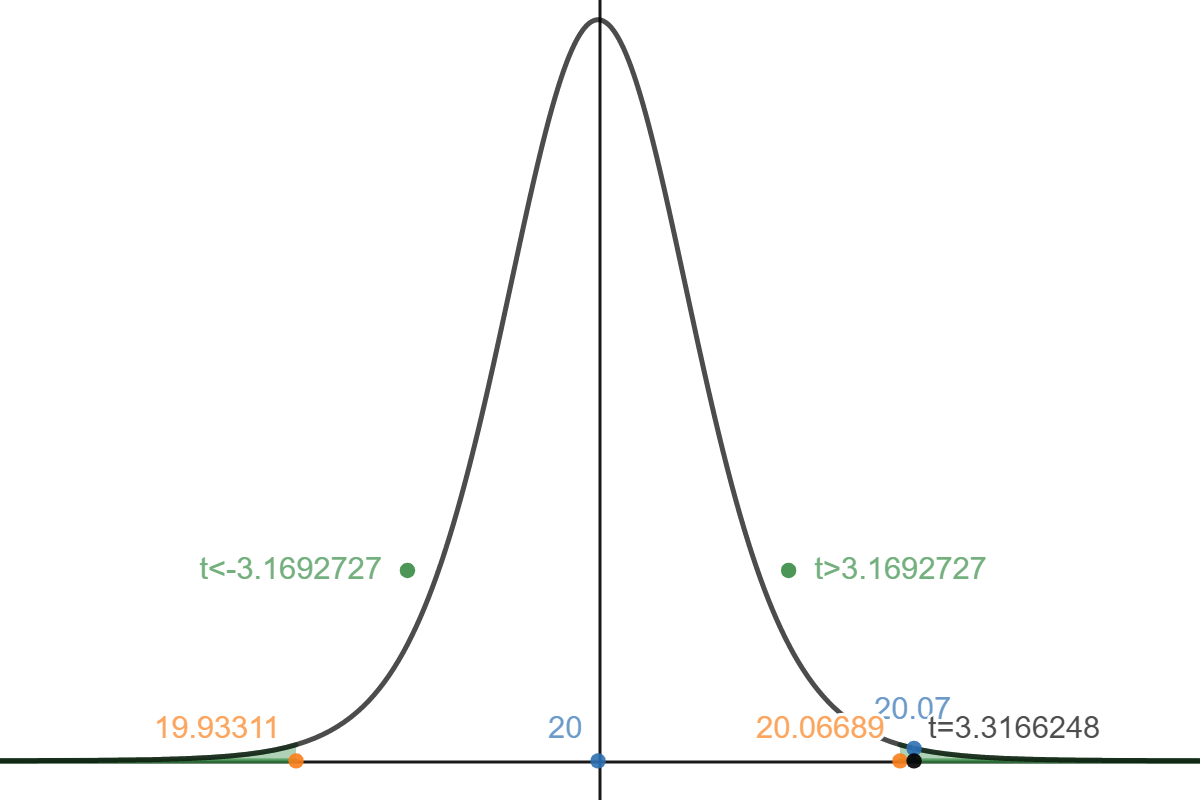
\includegraphics[scale=0.35]{2c_new.png}
\end{center}

\newpage

\section*{Answer 3}

\subsection*{Part a)}
Null hypothesis is: Difference of mean durations is 0 minutes.
$$H_0 : \mu_X - \mu_Y = 0$$

\subsection*{Part b)}
Alternate hypothesis is: Difference of mean durations is less then 0 minutes. ($\mu_X$ is better.)
$$H_A : \mu_X - \mu_Y < 0$$

\subsection*{Part c)}
Since level of significance is 5\%, $\alpha$ is $0.05$. We will use \textit{left-tail Z-test} since knowing if the duration is below $0$ is enough, so $z_{\alpha} = 1.645$.
$$Z = \frac{\overline{X} - \overline{Y} - D}{\sqrt{\frac{\sigma_X^2}{n} + \frac{\sigma_Y^2}{m}}} = \frac{2.8 - 3 - 0}{\sqrt{\frac{1.7^2}{68} + \frac{1.4^2}{68}}} = \frac{-0.2}{0.267} = -0.749$$

Since $Z > -Z_{\alpha}$, it is in the accepting area so we accept the null hypothesis. Thus, we conclude that the new painkiller does not produce better results.

\vspace{0.5cm}

\begin{center}
    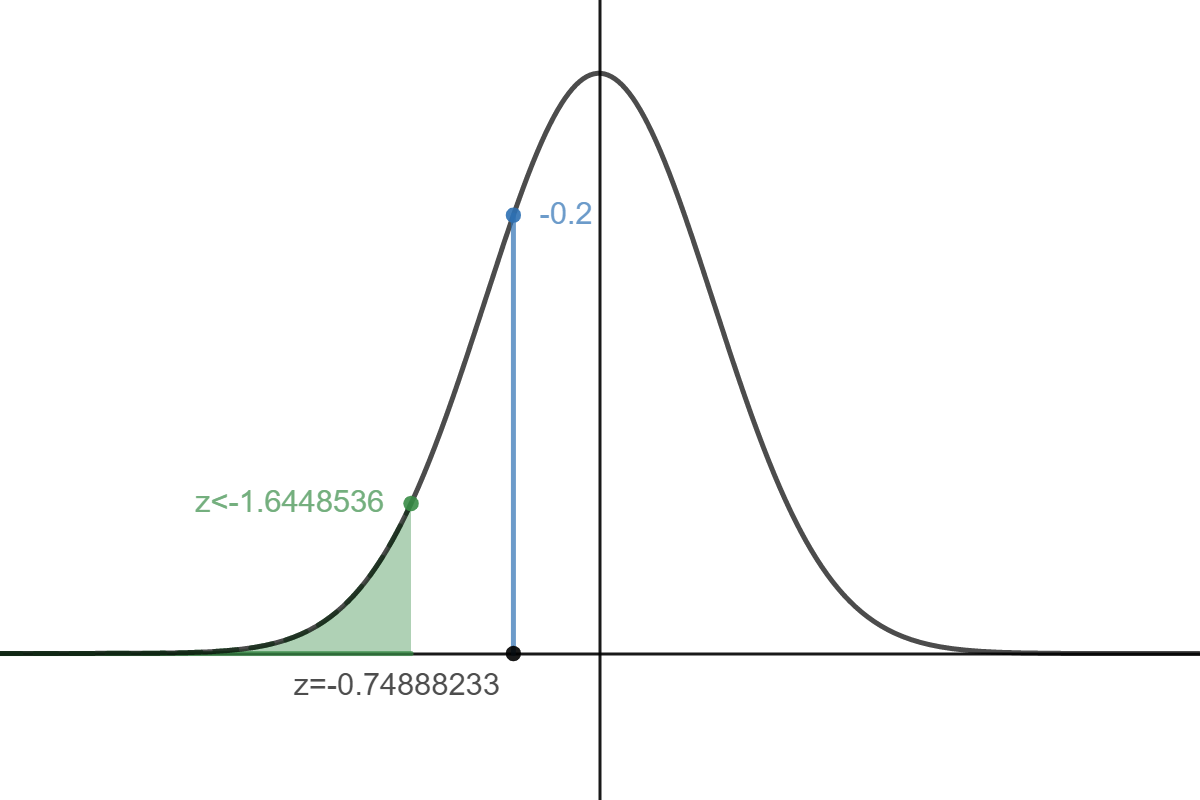
\includegraphics[scale=0.35]{3c_new.png}
\end{center}

\end{document}

